%%%%% fs-run-time-impl   Implementation

\label  {fs-implementation-section}

\subsection{Grouping semantics}
The grouping operation was defined in the previous section. Particularly, we assumed that data items get in grouping in the order provided by the global time. However, this restriction is hard to satisfy in our model, because it supports cycles. Therefore, our implementation of grouping satisfies two conditions:

\begin{enumerate}
\item All correct tuples are eventually produced.
\item Only a limited number of invalid tuples can be generated.
\end{enumerate}

The correctness of tuple means that this tuple would be generated if the order assumption was satisfied. 

As it was mentioned, grouping stores all input items in buckets by the value of hash function. Since the order of input items is arbitrary, we can only maintain the order of items within buckets. Hence, our implementation of grouping semantics includes two steps, which are detailed in the next two subsections. The way to prevent outputting wrong tuples from sink is described further.

\subsubsection{Invalidation}
Our implementation of grouping semantics requires replaying of tuples, which is described in details in the next subsection. However, now we should notice that replaying can generate tuples with the same global time. Because of the cycles, such items can get in grouping. Therefore, there is a need to remove them from the buckets, because they can produce an unbounded number of invalid tuples. To achieve this goal we introduce the invalidation relation between two data items. Therefore, if new item {\it B} invalidates item {\it A}, item {\it B} replaces item {\it A} in the bucket.

The data item {\it A} is said to be invalidated by the data item {\it B} if:
\begin{enumerate}
\item They have the same global time
\item The trace of {\it A} is less than the trace of {\it B}
\item The first difference is in logical time
\end{enumerate}
If the first difference is in child id, i.e. the items are brothers, there is no invalidation relation between them. Hence, the invalidation relation is a partial order.

Notably, the invalidation relation cannot be lost, when item is go through other operations, because the trace of local times is append-only. This property is applied further to invalidate items before they get in sink.

\subsubsection{Replaying}

Replaying is used to eventually produce all correct tuples. If the item gets in grouping, according to the global time order, nothing is replayed. If the item is out-of-order and/or it invalidates other item, then all tuples, which contain this element, are reproduced. The example of invalidation and replaying is shown on the figure~\ref{grouping-invalidation-figure}. In this example the green item is out-of-order and, moreover, it invalidates red item.

Thereby, replaying guarantees that eventually all correct tuples are produced. At the same time invalidation prevents from producing the unbounded number of incorrect tuples. 

\begin{figure}[htbp]
  \centering
  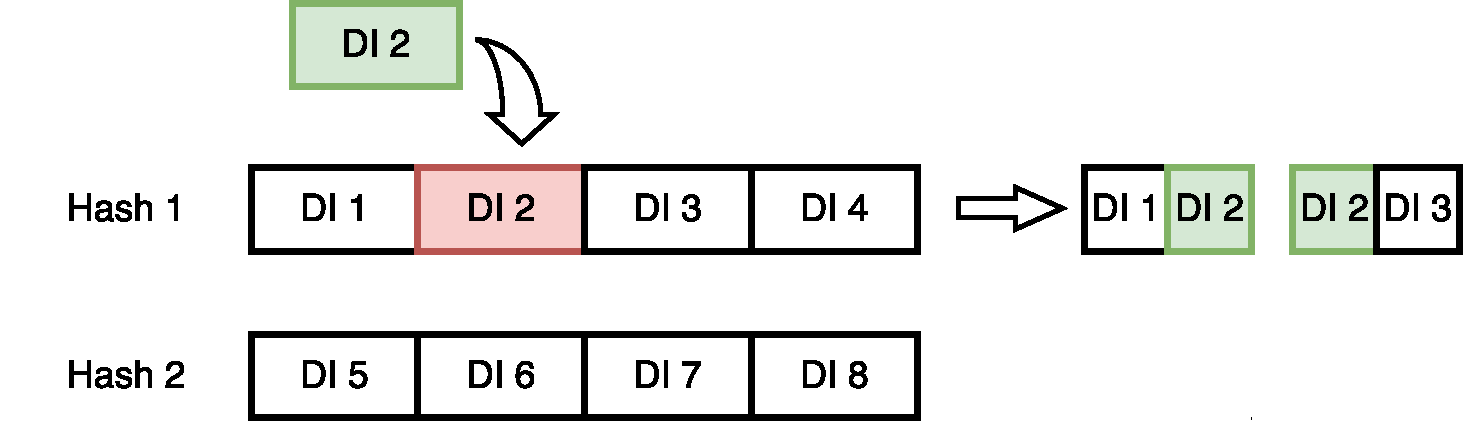
\includegraphics[width=0.48\textwidth]{pics/grouping-invalidation}
  \caption{Invalidation and replaying in grouping}
  \label {grouping-invalidation-figure}
\end{figure}

\subsection{Physical deployment and partitioning}

Each node in our distributed runtime is assigned by integer interval. Intervals are not intersected and cover the range of 32-bit signed integer. Moreover, each node contains complete logical graph.

As it was mentioned in the previous section, logical graph does not provide information about physical deployment. Physical graph extends logical one by assigning hash function to each operation. This hash function is applied to the payload of data items and determines partitioning. More precisely, the value of hash function is computed before each operation and corresponding data item is sent to the node which is responsible for the computed value. Therefore, load balancing explicitly depends on the hash functions of the operations. Optimal balancing requires the knowledge of payload distribution. Hence, the hash functions are assigned by business logic.

Notably, the hash function within grouping should be the same as partitioning hash function for grouping, because it guarantees that the result does not depend on the physical graph deployment.

Figure~\ref{logical-graph-figure} shows the example workflow of logical graph. Possible partitioning of this logical graph on two nodes is shown on the figure~\ref{physical-graph-figure}.

\begin{figure}[htbp]
  \centering
  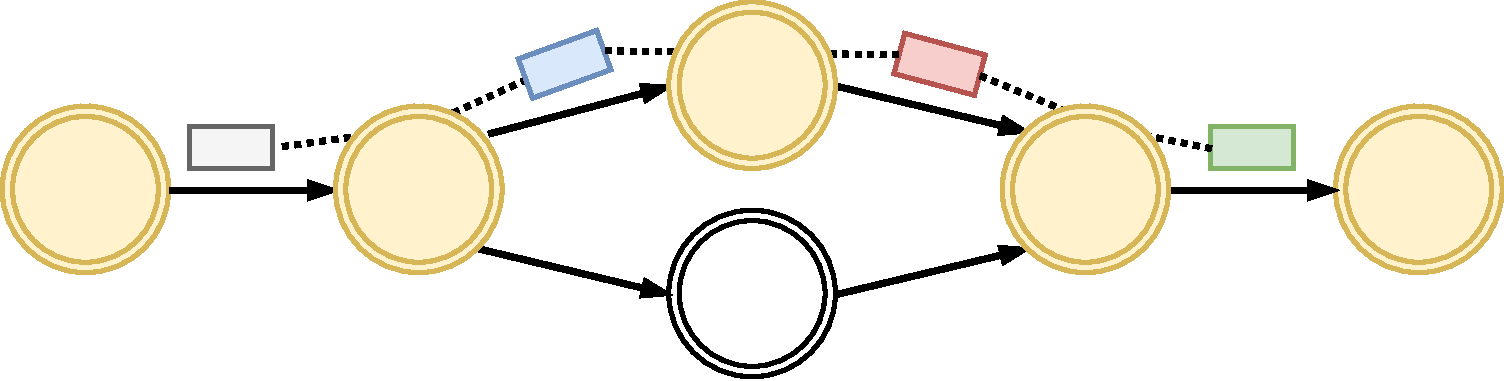
\includegraphics[width=0.48\textwidth]{pics/logical-graph}
  \caption{Logical graph workflow}
  \label {logical-graph-figure}
\end{figure}

\begin{figure}[htbp]
  \centering
  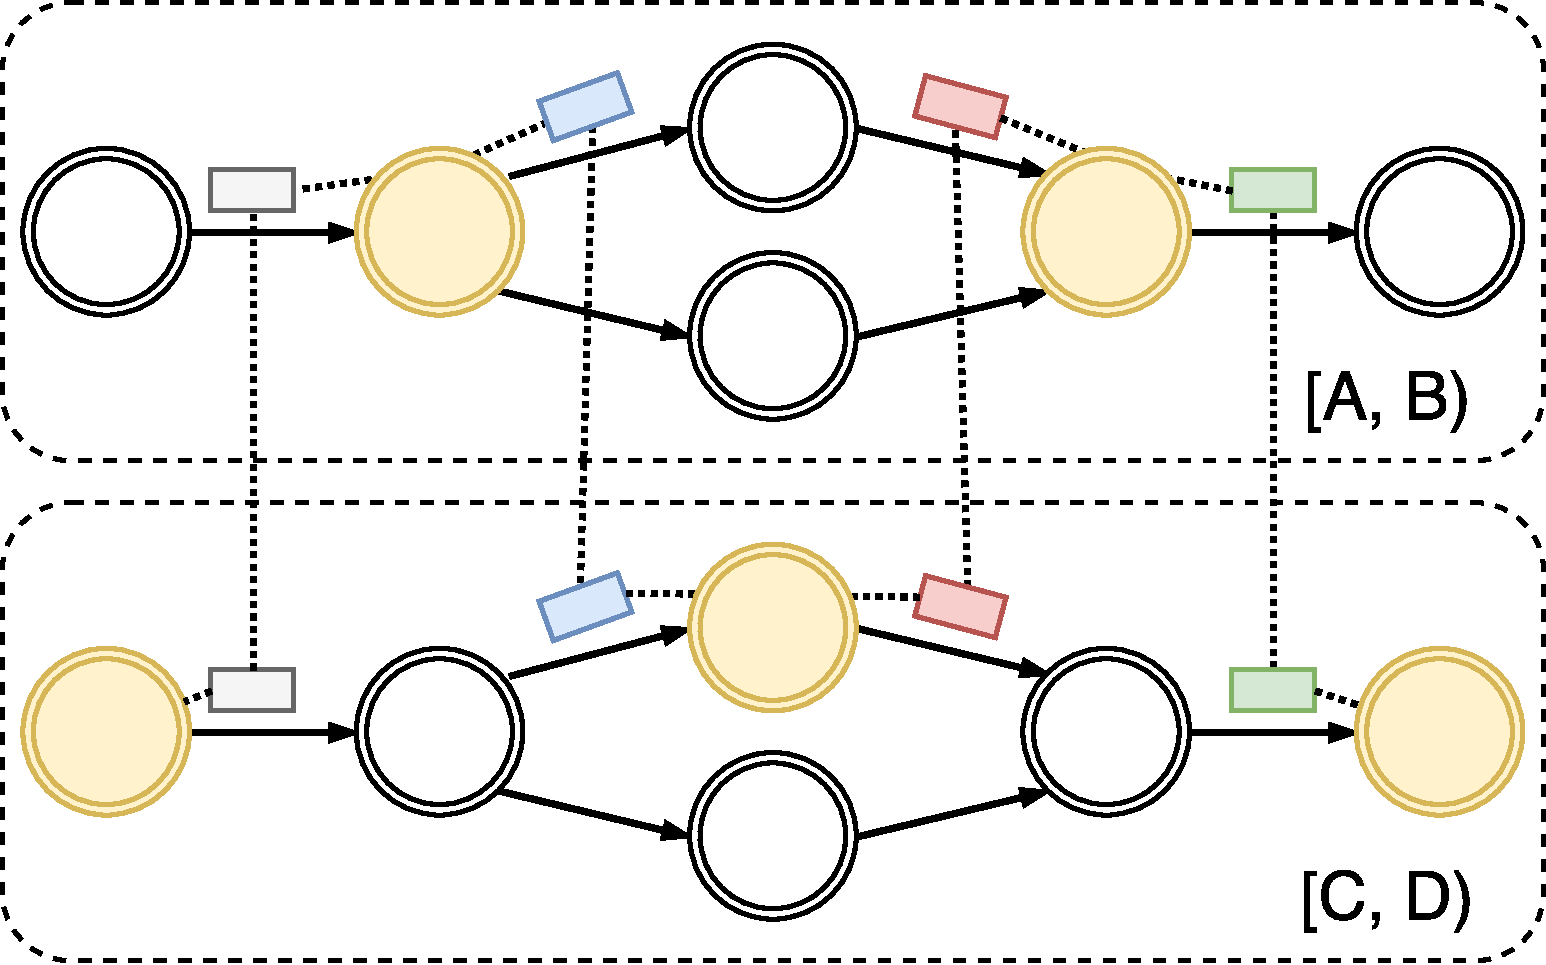
\includegraphics[width=0.48\textwidth]{pics/physical-graph}
  \caption{Possible partitioning of the logical graph}
  \label {physical-graph-figure}
\end{figure}

\subsection{System barriers}

\subsubsection{Front}
Front plays the role of data source. We assume that link between client's data and front is reliable and stable. The failure of this link is considered as the failure of client.

When data payloads are arrived to front, meta-information is assigned to them. As soon as the data obtains its meta-information, it is supposed that the system is responsible for this data. 

Each front is connected to corresponding operation. Similarly to the common physical graph vertex, data is sent to the appropriate node according to the value of hash function. Figure <> shows the example of interaction between client, front, and the other graph components.

\subsubsection{Sink}
Sink is the last node in any graph. It contains a buffer for data items. The items from buffer are released at some points in time. As it was mentioned above, grouping operation can generate invalid items. Consequently, there is a need to remove them from buffer before they get out from the system.  

However, there are two main difficulties. Firstly, sinks are the parts of the physical graph, so they are also partitioned by the business-logic hash function. Hence, item and corresponding invalidation item can arrive to distinct sinks. This issue can be solved by use of special partitioning for sinks by global time. Secondly, it is unclear when the items should be released from the buffer. To do it the system should ensure that there are no in-flight items which can invalidate items in buffer. The solution of this problem is detailed in the next section. 

Figure~\ref{invalidation-problems-figure} illustrates possible sink issues. Red items with labels 4 and 7 got out from the system, despite the fact that they should be invalidated by corresponding green items. 

\begin{figure}[htbp]
  \centering
  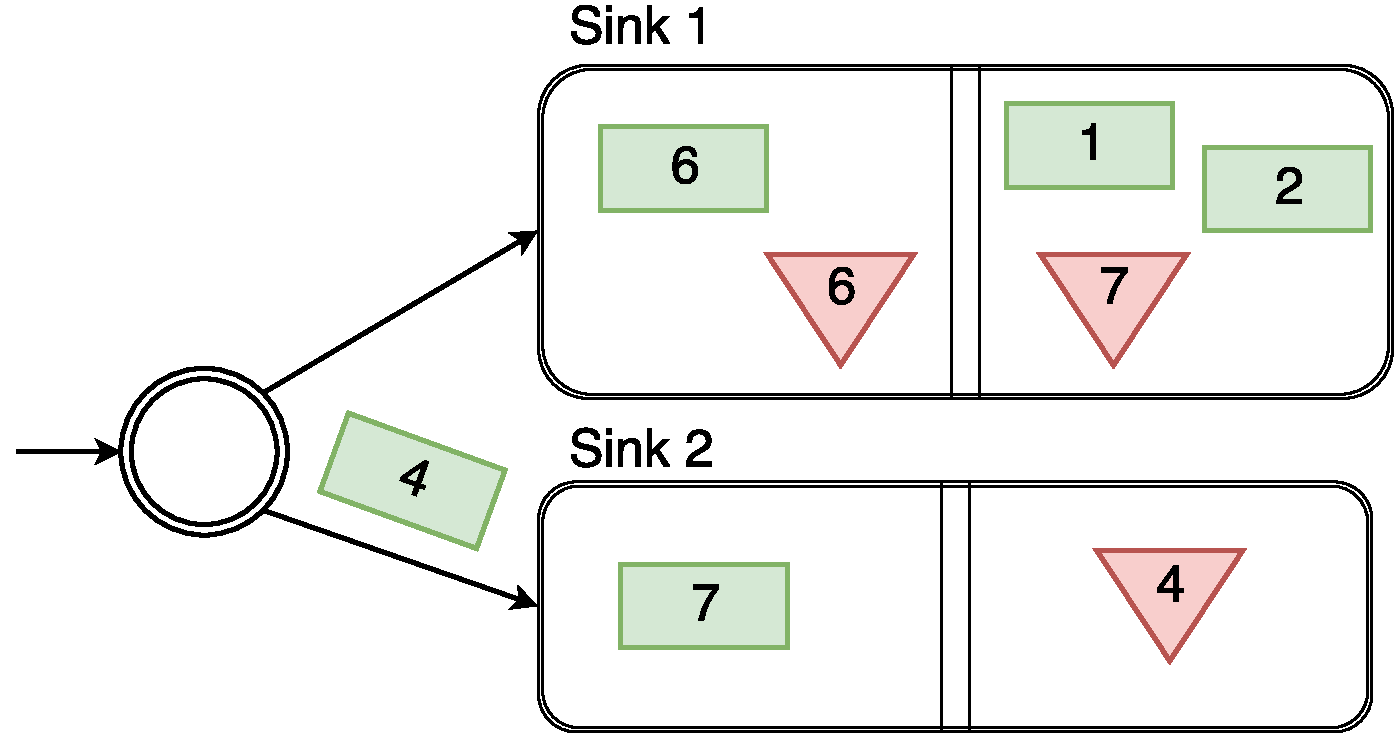
\includegraphics[width=0.48\textwidth]{pics/invalidation_problems}
  \caption{Possible sink issues}
  \label {invalidation-problems-figure}
\end{figure}

\subsection{Minimal time within stream}
Minimal time within stream is similar to Low watermark concept used in MillWheel~\cite{Akidau:2013:MFS:2536222.2536229}

Minimal time = Low watermark

OnMinTime = Timer trigger

\subsection{Fault-tolerance}

\subsubsection{State management}
Upon commit grouping saves a copy of its state on disk. To avoid pipeline blockage it can be done asynchronous to new data arrival. Check section 4.2 of \cite{Carbone:2017:SMA:3137765.3137777}

Not implemented yet but our architecture allows up to do so. 

Should we write about smth that isn't ours contribution?

\subsection{Guarantees}

\subsubsection{At least once}
On min time: State + replay + determinism = At least once

\subsubsection{Exactly once}
On min time: State + replay + determinism + idempotent sink = Exactly once

On commit: State + replay = Exactly once



